\documentclass[portrait,a0,final]{a0poster}

\usepackage[includeheadfoot,top=18mm,bottom=18mm,left=22mm,right=22mm,headsep=0mm,footskip=0mm]{geometry}
\usepackage[T1]{fontenc}
\usepackage[utf8]{inputenc}
\usepackage[scaled=.96]{helvet}
\renewcommand{\familydefault}{\sfdefault}
\usepackage{microtype}
\usepackage[table]{xcolor}
\usepackage{tikz}
\usetikzlibrary{arrows.meta,positioning,calc}
\usepackage{tabularx}
\usepackage{array}
\usepackage{booktabs}
\usepackage{amsmath}
\usepackage[most]{tcolorbox}
\usepackage{ragged2e}

\pagestyle{empty}
\setlength{\parindent}{0pt}
\setlength{\parskip}{3pt}
\renewcommand{\arraystretch}{1.14}

% EPFL-inspired palette. The layout uses the A0 poster class and sizing files
% from the supplied LaTeX template, with EPFL course branding.
\definecolor{epflred}{HTML}{E30613}
\definecolor{ink}{HTML}{111111}
\definecolor{muted}{HTML}{58606A}
\definecolor{softgray}{HTML}{F2F3F5}
\definecolor{linegray}{HTML}{D8DDE4}
\definecolor{softred}{HTML}{FDE7EA}
\definecolor{softblue}{HTML}{EAF2FB}
\definecolor{softgreen}{HTML}{EAF7EF}
\definecolor{softamber}{HTML}{FFF3DD}
\definecolor{blue}{HTML}{2B71B9}
\definecolor{green}{HTML}{2F8F57}
\definecolor{amber}{HTML}{C77D10}
\definecolor{deepred}{HTML}{A00008}
\definecolor{posterbg}{HTML}{FFFFFF}

\pagecolor{posterbg}
\color{ink}

\newcommand{\logofont}{\fontsize{78}{82}\selectfont}
\newcommand{\titlefont}{\fontsize{56}{64}\selectfont}
\newcommand{\subtitlefont}{\fontsize{28}{34}\selectfont}
\newcommand{\sectionfont}{\fontsize{29}{34}\selectfont}
\newcommand{\bodyfont}{\fontsize{21.5}{27}\selectfont}
\newcommand{\smallfont}{\fontsize{16.5}{20.5}\selectfont}
\newcommand{\tinyfont}{\fontsize{12.8}{16}\selectfont}
\newcommand{\tablefont}{\fontsize{13.5}{16.5}\selectfont}
\newcommand{\captionfont}{\fontsize{14}{17}\selectfont}

\newcolumntype{Y}{>{\RaggedRight\arraybackslash}X}
\newcolumntype{L}[1]{>{\RaggedRight\arraybackslash}p{#1}}
\newcolumntype{C}[1]{>{\centering\arraybackslash}p{#1}}
\newcolumntype{R}[1]{>{\RaggedLeft\arraybackslash}p{#1}}

\newtcolorbox{panelbox}[1][]{
  enhanced,
  colback=softgray,
  colframe=softgray,
  boxrule=0pt,
  sharp corners,
  left=6mm,
  right=6mm,
  top=5mm,
  bottom=5mm,
  before skip=0mm,
  after skip=0mm,
  #1
}

\newtcolorbox{whitebox}[1][]{
  enhanced,
  colback=white,
  colframe=linegray,
  boxrule=0.8pt,
  sharp corners,
  left=4mm,
  right=4mm,
  top=3mm,
  bottom=3mm,
  before skip=0mm,
  after skip=0mm,
  #1
}

\newtcolorbox{callout}[2]{
  enhanced,
  colback=#2,
  colframe=#1,
  boxrule=0.9pt,
  sharp corners,
  left=4mm,
  right=4mm,
  top=3mm,
  bottom=3mm,
  before skip=2mm,
  after skip=2mm
}

\newcommand{\blockhead}[2]{%
  \noindent
  \tikz[baseline=(n.base)]{
    \node[fill=epflred,text=white,rounded corners=1mm,
      inner xsep=3.2mm,inner ysep=1.7mm,
      font=\bfseries\sectionfont] (n) {#1};
    \node[anchor=west,text=epflred,font=\bfseries\sectionfont]
      at ([xshift=4mm]n.east) {#2};
  }\par\vspace{3mm}
}

\newcommand{\tightitems}{%
  \setlength{\itemsep}{2.2mm}
  \setlength{\topsep}{1mm}
  \setlength{\parsep}{0mm}
  \setlength{\partopsep}{0mm}
}

\newcommand{\scorebar}[3]{%
  \begin{tikzpicture}[x=1mm,y=1mm,baseline=-0.5ex]
    \draw[fill=white,draw=white] (0,0) rectangle (116,8);
    \draw[fill=#2,draw=#2] (0,0) rectangle ({116*#1},8);
    \node[anchor=west,font=\bfseries\smallfont] at (121,4) {#3};
  \end{tikzpicture}
}

\newcommand{\metricpill}[4]{%
  \begin{whitebox}[colframe=#3,colback=#4,height=39mm]
    {\bfseries #1}\\[-1mm]
    {\smallfont #2}
  \end{whitebox}
}

\begin{document}
\bodyfont

% Header
\begin{minipage}[t]{0.22\textwidth}
  {\logofont\bfseries\color{epflred}EPFL}
\end{minipage}
\hfill
\begin{minipage}[t]{0.50\textwidth}
  \raggedleft
  {\smallfont Law and Computation II \, | \, Capstone Project Poster Presentation\\
  Spring 2026 \, | \, A0 portrait}
\end{minipage}

\vspace{7mm}

% Title band
\begin{tcolorbox}[
  enhanced,
  colback=epflred,
  colframe=epflred,
  boxrule=0pt,
  sharp corners,
  left=11mm,
  right=11mm,
  top=11mm,
  bottom=10mm
]
{\titlefont\bfseries\color{white} Formalizing Copyright Law Through Melody Similarity}\\[4mm]
{\subtitlefont\color{white} An explainable decision-support prototype for music copyright disputes}\\[5mm]
{\smallfont\color{white} Ryad Mohamed Aouak, Romain Greub, Gresi Alejandra Velasco-Miranda, Zichun Zhou}
\end{tcolorbox}

\vspace{5mm}

\begin{callout}{epflred}{softred}
{\subtitlefont\bfseries Project claim.}
\hspace{3mm}
{\bodyfont\bfseries We do not automate copyright adjudication. We make one legally relevant issue explicit and inspectable: whether two songs share a recognizable melodic fragment.}
\end{callout}

\vspace{7mm}

% Row 1
\begin{minipage}[t]{0.318\textwidth}
\begin{panelbox}[height=166mm]
\blockhead{1}{Legal Problem}
Music copyright disputes often turn on the open-textured standard of
\textbf{substantial similarity}. But similarity is not itself a legal conclusion.

\begin{itemize}
\tightitems
\item Courts also consider access, protectability, scope of the disputed material, and context.
\item Raw similarity scores can be persuasive but legally misleading if their meaning is hidden.
\item The research gap is not only computational; it is techno-legal: how can a score support legal reasoning without pretending to replace it?
\end{itemize}

\begin{callout}{epflred}{softred}
\textbf{Research question.}
Can local melodic alignment capture legally relevant fragment similarity better than global comparison while remaining explainable enough for decision support?
\end{callout}
\end{panelbox}
\end{minipage}
\hfill
\begin{minipage}[t]{0.318\textwidth}
\begin{panelbox}[height=166mm]
\blockhead{2}{Achieved Scope}
The fall pitch proposed a broad formalization pipeline. The implemented poster-stage prototype focuses on the part that can be defended with the current code and data.

\vspace{2mm}
\begin{tabularx}{\linewidth}{@{}L{0.36\linewidth}Y@{}}
\toprule
\textbf{Initial ambition} & \textbf{Achieved component}\\
\midrule
Legal formalization & Minimal legal variables and rule-trace logic.\\
Similarity layer & Global PMI, local PMI, and hybrid PMI.\\
Threshold analysis & Exploratory thresholds on 15 melody-dispute pairs.\\
Decision support & Scorecard interpretation, not automated judgment.\\
\bottomrule
\end{tabularx}

\vspace{3mm}
\begin{callout}{blue}{softblue}
\textbf{Why this is credible.}
The poster presents the working evidence layer clearly: what it measures, where it helps, and where legal judgment must remain in control.
\end{callout}
\end{panelbox}
\end{minipage}
\hfill
\begin{minipage}[t]{0.318\textwidth}
\begin{panelbox}[height=166mm]
\blockhead{3}{Dataset and Legal Coding}
\begin{tabularx}{\linewidth}{@{}L{0.36\linewidth}Y@{}}
\toprule
\textbf{Artifact} & \textbf{Current state}\\
\midrule
Corpus & 128 music copyright disputes in the master case file.\\
Evaluation subset & 15 pairs with curated MIDI melody excerpts.\\
Representation & Monophonic pitch sequences converted to intervals.\\
Legal variables & Access, melody scope, protectability, context override.\\
\bottomrule
\end{tabularx}

\vspace{4mm}
\begin{callout}{green}{softgreen}
\textbf{Bounded contribution.}
The project is strongest when presented as an explainable similarity and legal-interpretation layer for melody-focused cases.
\end{callout}
\end{panelbox}
\end{minipage}

\vspace{9mm}

% Row 2: method overview
\begin{panelbox}[height=218mm]
\blockhead{4}{Method Overview}
\begin{minipage}[t]{0.685\linewidth}
\textbf{Implemented pipeline.} MIDI melody excerpts are transformed into interval sequences, aligned globally and locally, then interpreted through a minimal legal rule layer.

\vspace{5mm}
\begin{center}
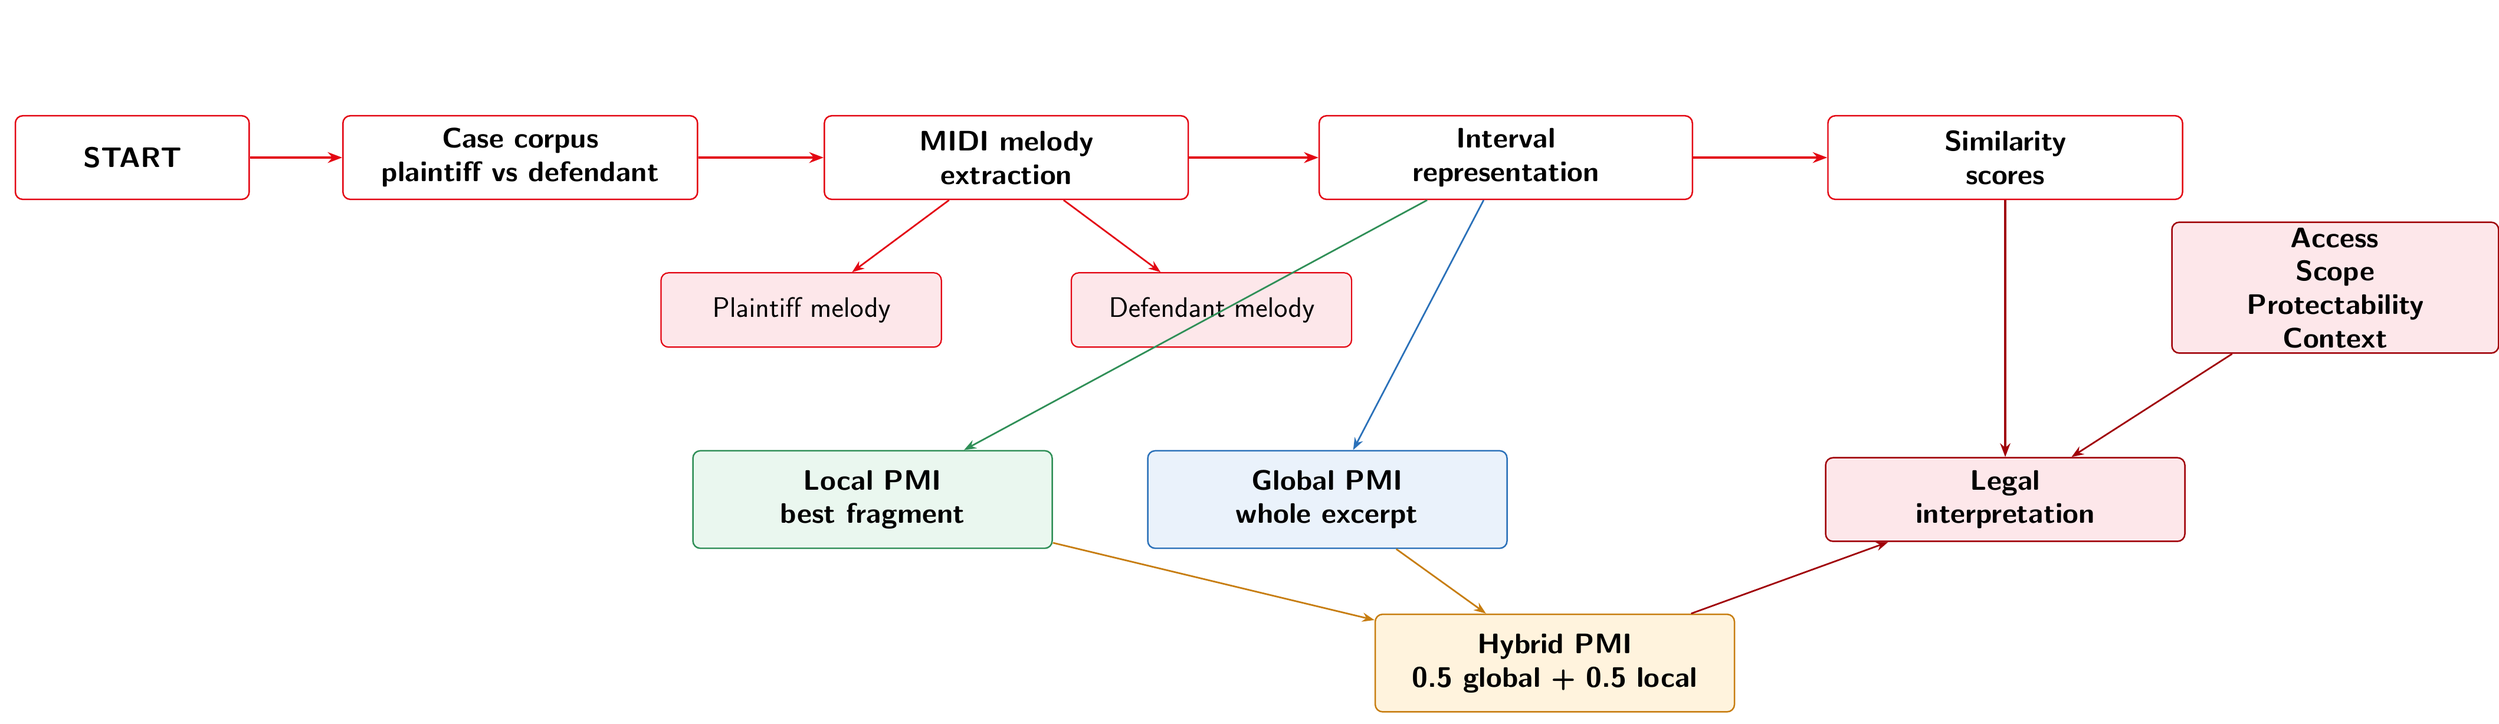
\begin{tikzpicture}[x=0.96mm,y=0.80mm,>=Stealth,transform shape]
  \path[use as bounding box] (-8,-98) rectangle (545,88);
  \tikzset{
    main/.style={draw=epflred,fill=white,line width=0.9pt,rounded corners=1.6mm,align=center,font=\bfseries\smallfont,minimum height=18mm},
    sub/.style={draw=epflred,fill=softred,line width=0.8pt,rounded corners=1.6mm,align=center,font=\smallfont,minimum height=16mm},
    bluebox/.style={draw=blue,fill=softblue,line width=0.9pt,rounded corners=1.6mm,align=center,font=\bfseries\smallfont,minimum height=21mm},
    greenbox/.style={draw=green,fill=softgreen,line width=0.9pt,rounded corners=1.6mm,align=center,font=\bfseries\smallfont,minimum height=21mm},
    amberbox/.style={draw=amber,fill=softamber,line width=0.9pt,rounded corners=1.6mm,align=center,font=\bfseries\smallfont,minimum height=21mm},
    lawbox/.style={draw=deepred,fill=softred,line width=0.9pt,rounded corners=1.6mm,align=center,font=\bfseries\smallfont,minimum height=18mm}
  }
  \node[main,text width=48mm] (start) at (18,50) {START};
  \node[main,text width=74mm] (corpus) at (105,50) {Case corpus\\plaintiff vs defendant};
  \node[main,text width=76mm] (midi) at (214,50) {MIDI melody\\extraction};
  \node[main,text width=78mm] (interval) at (326,50) {Interval\\representation};
  \node[main,text width=74mm] (score) at (438,50) {Similarity\\scores};
  \node[lawbox,text width=75mm] (legal) at (438,-42) {Legal\\interpretation};

  \node[sub,text width=58mm] (p) at (168,9) {Plaintiff melody};
  \node[sub,text width=58mm] (d) at (260,9) {Defendant melody};
  \node[bluebox,text width=75mm] (global) at (286,-42) {Global PMI\\whole excerpt};
  \node[greenbox,text width=75mm] (local) at (184,-42) {Local PMI\\best fragment};
  \node[amberbox,text width=75mm] (hybrid) at (337,-86) {Hybrid PMI\\0.5 global + 0.5 local};
  \node[lawbox,text width=68mm] (access) at (512,15) {Access\\Scope\\Protectability\\Context};

  \draw[->,line width=1.3pt,epflred] (start) -- (corpus);
  \draw[->,line width=1.3pt,epflred] (corpus) -- (midi);
  \draw[->,line width=1.3pt,epflred] (midi) -- (interval);
  \draw[->,line width=1.3pt,epflred] (interval) -- (score);
  \draw[->,line width=1.0pt,epflred] (midi) -- (p);
  \draw[->,line width=1.0pt,epflred] (midi) -- (d);
  \draw[->,line width=1.0pt,green] (interval) -- (local);
  \draw[->,line width=1.0pt,blue] (interval) -- (global);
  \draw[->,line width=1.0pt,amber] (global) -- (hybrid);
  \draw[->,line width=1.0pt,amber] (local) -- (hybrid);
  \draw[->,line width=1.2pt,deepred] (score) -- (legal);
  \draw[->,line width=1.0pt,deepred] (access) -- (legal);
  \draw[->,line width=1.0pt,deepred] (hybrid) -- (legal);
\end{tikzpicture}
\end{center}
\end{minipage}
\hfill
\begin{minipage}[t]{0.292\linewidth}
\textbf{Melody representation.}
\[
I=[p_2-p_1,\;p_3-p_2,\ldots,p_n-p_{n-1}]
\]
Intervals make comparison key-invariant and focused on melodic contour.

\vspace{4mm}
\metricpill{Global PMI}{Whole-excerpt resemblance. Conservative, but rigid when copying is fragment-based.}{blue}{softblue}
\vspace{3mm}
\metricpill{Local PMI}{Best-matching fragment resemblance. Closer to legally relevant motif copying.}{green}{softgreen}
\vspace{3mm}
\metricpill{Hybrid PMI}{Balances whole-melody and fragment evidence so one local match does not decide the case alone.}{amber}{softamber}
\end{minipage}

\end{panelbox}

\vspace{9mm}

% Row 3: results
\begin{panelbox}[height=286mm]
\blockhead{5}{Results}
\begin{minipage}[t]{0.355\linewidth}
\textbf{Threshold behavior on 15 curated melody pairs.}

\vspace{4mm}
\begin{tabularx}{\linewidth}{@{}L{0.25\linewidth}Y@{}}
Global $>20\%$ & \scorebar{0.267}{blue}{4/15}\\[4mm]
Local $>80\%$ & \scorebar{0.733}{green}{11/15}\\[4mm]
Hybrid $>50\%$ & \scorebar{0.600}{amber}{9/15}\\
\end{tabularx}

\vspace{7mm}
\begin{callout}{green}{softgreen}
\textbf{Main empirical finding.}
Local PMI detects substantially more known fragment-based disputes than global PMI.
\end{callout}
\begin{callout}{epflred}{softred}
\textbf{Legal caution.}
High similarity is over-inclusive: a score needs access, protectability, scope, and context before it becomes legally meaningful.
\end{callout}

\vspace{4mm}
\begin{whitebox}[height=78mm]
\textbf{Illustrative readings.}\\[1mm]
{\smallfont
\begin{tabularx}{\linewidth}{@{}Y R{0.18\linewidth} R{0.18\linewidth}@{}}
\toprule
\textbf{Pair} & \textbf{G} & \textbf{L}\\
\midrule
No Scrubs / Shape of You & 8.39 & 92.12\\
Bitter Sweet Symphony / The Last Time & 26.95 & 77.54\\
Ice Ice Baby / Under Pressure & 2.78 & 33.33\\
Flowers / When I Was Your Man & 36.10 & 89.43\\
\bottomrule
\end{tabularx}}
\end{whitebox}
\end{minipage}
\hfill
\begin{minipage}[t]{0.615\linewidth}
\textbf{Full score table.} Global and local scores are shown separately; the hybrid score is their simple average.

\vspace{3mm}
{\tablefont
\begin{tabularx}{\linewidth}{@{}C{0.055\linewidth}Y R{0.105\linewidth} R{0.105\linewidth} R{0.115\linewidth}@{}}
\toprule
\rowcolor{white}
\textbf{\#} & \textbf{Melody pair} & \textbf{Global} & \textbf{Local} & \textbf{Hybrid}\\
\midrule
1 & The Last Time / Bitter Sweet Symphony & 26.95 & 77.54 & 52.24\\
2 & Anybody Seen My Baby / Constant Craving & 5.01 & 93.08 & 49.04\\
3 & All You Need Is Love / In the Mood & 12.85 & 95.05 & 53.95\\
4 & Oops Up Side Your Head / Uptown Funk & 6.58 & 62.90 & 34.74\\
5 & Greatest Love of All / If You Could Read My Mind & 21.10 & 93.23 & 57.16\\
6 & Sweet Little Sixteen / Surfin' U.S.A. & 18.62 & 93.70 & 56.16\\
7 & I Won't Back Down / Stay With Me & 7.76 & 88.89 & 48.32\\
8 & No Scrubs / Shape of You & 8.39 & 92.12 & 50.25\\
9 & I'm Not Alone / Yeah 3x & 3.61 & 0.00 & 1.81\\
10 & Teach the World to Sing / Shakermaker & 12.90 & 89.46 & 51.18\\
11 & Under Pressure / Ice Ice Baby & 2.78 & 33.33 & 18.06\\
12 & Every Breath You Take / I'll Be Missing You & 23.01 & 93.35 & 58.18\\
13 & All Day and All of the Night / Hello, I Love You & 12.74 & 93.94 & 53.34\\
14 & I Want a New Drug / Ghostbusters & 9.91 & 85.00 & 47.45\\
15 & When I Was Your Man / Flowers & 36.10 & 89.43 & 62.77\\
\bottomrule
\end{tabularx}}

\vspace{4mm}
\begin{callout}{blue}{softblue}
\textbf{Interpretation.}
Global PMI is useful as a conservative baseline; local PMI is better aligned with the legal intuition that a recognizable fragment can matter even when the full melodies differ.
\end{callout}
\end{minipage}
\par\vspace{6mm}
\begin{whitebox}[height=48mm]
\begin{minipage}[t]{0.31\linewidth}
{\bfseries\color{blue}Global result.}
Conservative whole-excerpt comparison flags only 4/15 pairs, so it misses several fragment-centered disputes.
\end{minipage}
\hfill
\begin{minipage}[t]{0.31\linewidth}
{\bfseries\color{green}Local result.}
Best-fragment comparison flags 11/15 pairs and better matches the way melody disputes are argued.
\end{minipage}
\hfill
\begin{minipage}[t]{0.31\linewidth}
{\bfseries\color{amber}Hybrid result.}
The combined score flags 9/15 pairs, keeping sensitivity while avoiding reliance on one fragment alone.
\end{minipage}
\end{whitebox}
\end{panelbox}

\vspace{9mm}

% Row 4: discussion and conclusion
\begin{minipage}[t]{0.318\textwidth}
\begin{panelbox}[height=193mm]
\blockhead{6}{Legal Interpretation}
The contribution is not that scores decide cases. The contribution is a transparent structure for interpreting scores.

\vspace{2mm}
\begin{tabularx}{\linewidth}{@{}L{0.34\linewidth}Y@{}}
\toprule
\textbf{Factor} & \textbf{Role}\\
\midrule
Access & Similarity is weaker without plausible access.\\
Melody scope & The tool should not decide lyrics, timbre, production, or vibe cases.\\
Protectability & High similarity can still concern generic material.\\
Context & Unusual cases require manual legal review.\\
\bottomrule
\end{tabularx}

\vspace{4mm}
\begin{callout}{amber}{softamber}
\textbf{Rule-trace logic.}
Stop if outside melodic scope; lower concern if access is absent; flag review only when similarity and legal factors align.
\end{callout}
\end{panelbox}
\end{minipage}
\hfill
\begin{minipage}[t]{0.318\textwidth}
\begin{panelbox}[height=193mm]
\blockhead{7}{Discussion}
\begin{itemize}
\tightitems
\item \textbf{Empirical:} local alignment better captures recognizable fragments than full-excerpt comparison.
\item \textbf{Legal:} similarity is evidence, not the legal test itself.
\item \textbf{Computational:} the model is interpretable because each score has a clear methodological meaning.
\item \textbf{Capstone value:} the work connects a measurable artifact to a legal reasoning structure.
\end{itemize}

\begin{callout}{green}{softgreen}
\textbf{Takeaway.}
Computation can clarify one part of copyright reasoning, but it should support human legal judgment rather than replace it.
\end{callout}
\end{panelbox}
\end{minipage}
\hfill
\begin{minipage}[t]{0.318\textwidth}
\begin{panelbox}[height=193mm]
\blockhead{8}{Conclusion}
\textbf{Final claim.}
The project achieved a defensible part of the original capstone goal: an explainable computational layer for melody-based copyright analysis.

\vspace{3mm}
\begin{tabularx}{\linewidth}{@{}L{0.39\linewidth}Y@{}}
\toprule
\textbf{Limitation} & \textbf{Next step}\\
\midrule
Melody only & Add rhythm, harmony, sampling, production.\\
15 MIDI pairs & Expand and balance evaluation.\\
Settlements as labels & Separate settlements from court findings.\\
Exploratory thresholds & Calibrate and report uncertainty.\\
Legal variables incomplete & Finish annotations and rule traces.\\
\bottomrule
\end{tabularx}
\end{panelbox}
\end{minipage}

\vspace{9mm}

\begin{tcolorbox}[
  enhanced,
  colback=epflred,
  colframe=epflred,
  boxrule=0pt,
  sharp corners,
  left=8mm,
  right=8mm,
  top=5mm,
  bottom=5mm
]
{\subtitlefont\bfseries\color{white} Final takeaway.}
\hspace{3mm}
{\bodyfont\bfseries\color{white} The prototype turns melodic similarity from a black-box number into auditable evidence: useful for legal reasoning, but never a substitute for legal judgment.}
\end{tcolorbox}

\vfill

% Footer
\begin{tcolorbox}[
  enhanced,
  colback=ink,
  colframe=ink,
  boxrule=0pt,
  sharp corners,
  left=7mm,
  right=7mm,
  top=4mm,
  bottom=4mm
]
{\tinyfont\color{white}
\textbf{References.}
Savage et al. (2018), \textit{Quantitative evaluation of music copyright infringement};
Needleman and Wunsch (1970), \textit{A general method applicable to sequence similarity};
Smith and Waterman (1981), \textit{Identification of common molecular subsequences};
Mullensiefen and Pendzich (2009), \textit{Court decisions on music plagiarism and the predictive value of similarity algorithms}.\\
\textbf{AI-use note.}
AI assistance was used for language, layout, and poster structuring; the authors remain responsible for all claims and presentation content.}
\end{tcolorbox}

\end{document}
